\resizebox{\columnwidth}{!}{
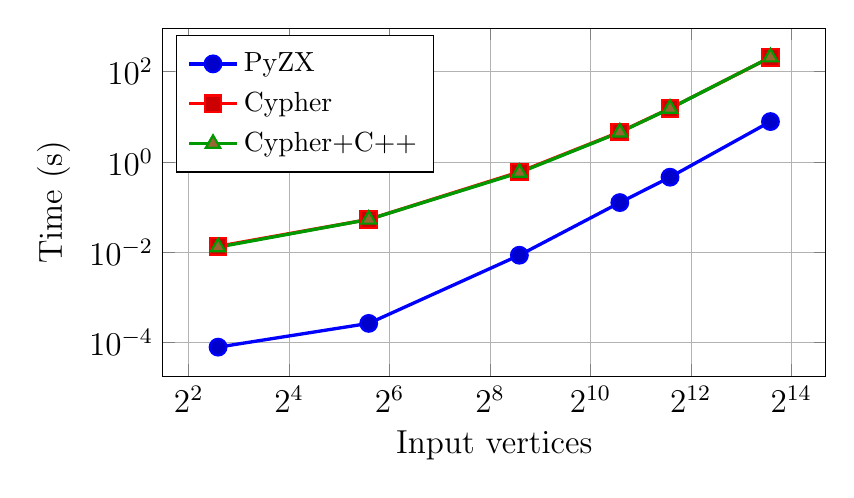
\begin{tikzpicture}
  \begin{axis}[
    width=10cm, height=6cm,
    xlabel={Input vertices}, ylabel={Time (s)},
    xmode=log, ymode=log, log basis x=2,
    grid=major,
    grid style={line width=.1pt, draw=gray!30},
    major grid style={line width=.2pt, draw=gray!60},
    label style={font=\large}, tick label style={font=\large},
    legend style={at={(0.02,0.98)}, anchor=north west,
      font=\normalsize, inner sep=4pt, row sep=2pt, cells={anchor=west}},
    legend image post style={mark size=3pt},
    every axis plot/.append style={line width=1.2pt, mark size=3pt,
      mark options={line width=0.8pt}},
    unbounded coords=jump,
  ]
    \addplot+[mark=*, color=blue, solid,error bars/.cd,y dir=both,y explicit] coordinates {
      (6,7.79000002e-05)
      (48,0.000261999998)
      (384,0.0085149)
      (1536,0.1252216)
      (3072,0.4580563)
      (12288,7.8473078)
    };
    \addlegendentry{PyZX}

    \addplot+[mark=square*, color=red, solid,error bars/.cd,y dir=both,y explicit] coordinates {
      (6,0.0134115)
      (48,0.0530501)
      (384,0.599007)
      (1536,4.6019953)
      (3072,15.4204163)
      (12288,208.651336)
    };
    \addlegendentry{Cypher}

    \addplot+[mark=triangle*, color=green!60!black, solid,error bars/.cd,y dir=both,y explicit] coordinates {
      (6,0.0129044)
      (48,0.0528197)
      (384,0.5784182)
      (1536,4.5331628)
      (3072,15.2592695)
      (12288,209.736774)
    };
    \addlegendentry{Cypher+C++}

  \end{axis}
\end{tikzpicture}
}
